\documentclass[xcolor=dvipsnames]{beamer} 

\usepackage[latin1]{inputenc}
\usefonttheme[onlymath]{serif}
\usepackage{amsmath}
\usepackage{amsfonts}
\usepackage{amssymb}
\usepackage{amsthm}
\usepackage{latexsym,float}
\usepackage{times}
\usepackage[T1]{fontenc}
\usepackage{lmodern}

\usepackage{amscd}
\usepackage{amsfonts}

\setbeamertemplate{footline}[page number]{}
\setbeamertemplate{navigation symbols}{}
\newtheorem{proposition}[theorem]{Proposition}

\usepackage{algorithm,algorithmic}
\definecolorset{rgb}{}{}{darkred,0.8,0,0;darkgreen,0,0.5,0;darkblue,0,0,0.5}

\title{Alignment of single-cell trajectories to compare cellular expression dynamics}
\author{Ayelet Alpert, Lindsay S Moore, Tania Dubovik \& Shai S Shen-Orr}
\date{Nature Methods (2018)}

\begin{document}

\setlength{\unitlength}{\textwidth}  % measure in textwidths

\frame{\titlepage}

\frame{
\frametitle{Background}

}

\frame{
\frametitle{Overview of cellAlign}
\begin{center}
	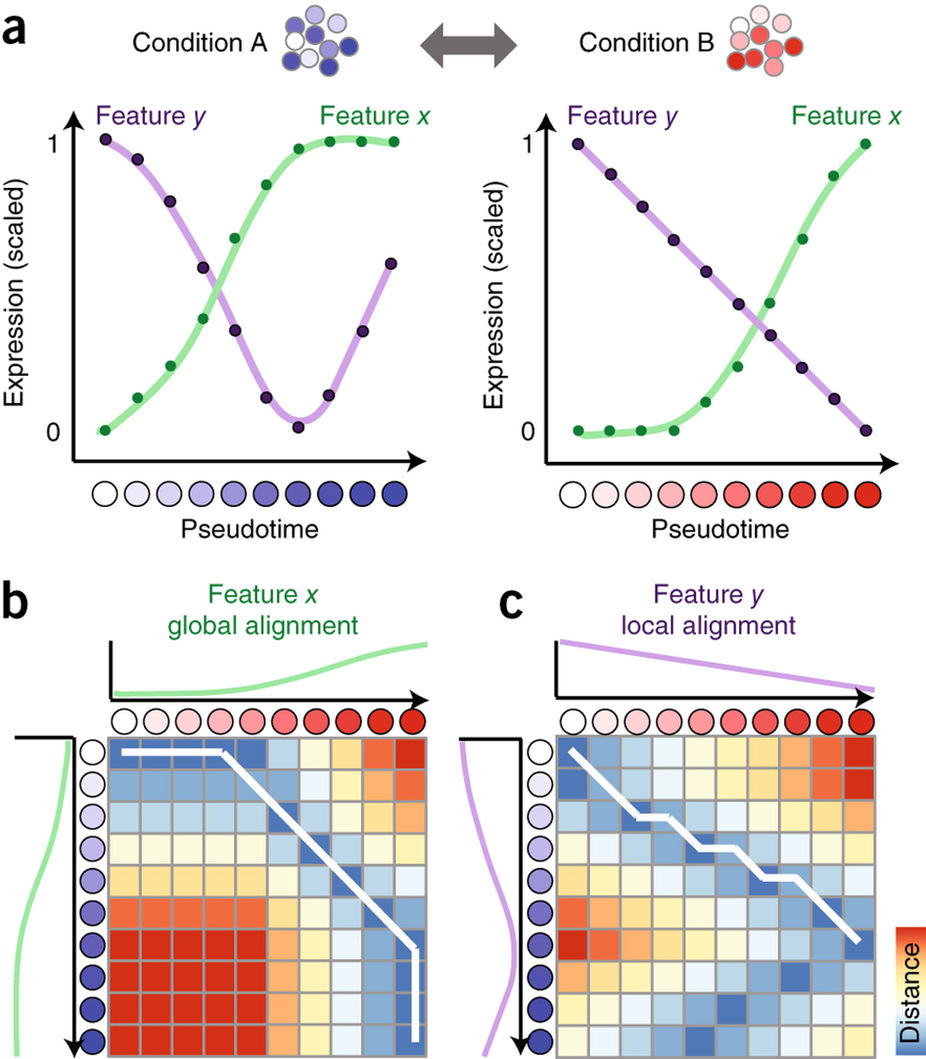
\includegraphics[width=0.5\textwidth]{Figures/F1}
\end{center}
}

\frame{
\frametitle{Methods: Interpolation}

}

\frame{
\frametitle{Methods: Dynamic time warping}

}

\frame{
\frametitle{Methods: Global alignment of expression dynamics}

}

\frame{
\frametitle{Methods: Local alignment of expression dynamics}

}

\frame{
\frametitle{Application: three trajectories from scRNA-seq generated independently}

}

\frame{
\frametitle{Benchmark: comparative analysis of dendritic cells' response to stimuli}

}

\frame{
\frametitle{Sensitivity analysis for random dropout events and preprocessing techniques}

}

\frame{
\frametitle{Application: differential temporal regulation between species}

}

\frame{
\frametitle{Application: difference in zygotic genome activation between mouse and human}

}


\frame{
\frametitle{Conclusion}
\begin{itemize}
	\item cellAlign compares expression dynamics along single cell trajectories describing different conditions (biological processes under different conditions)
	\item cellAlign preserves temporal resolution of single-cell trajecotries
	\item Other applications: mass cytometry proteomic data, robustness test of trajectory assembly algorithm to parameters and noises
\end{itemize}
}

\end{document}



%%%%%%%%%%%%%%%%%%%%%%%%%%%%%%%%%%%%%%%%%%%%%%%%%


\frame{
\frametitle{Motivation: Estimation of Effective Population Size}
Effective Population Size is a measure of \textcolor{darkgreen}{relative genetic diversity}.

\begin{center}
\includegraphics[width=0.9\textwidth]{../Rcode/presentationFigures/flu_vs_measles_coalescence}
\end{center}
\tiny{Bedford et al. BMC Evolutionary Biology 2011}
}


\frame{
\frametitle{Present-day molecular sequence data inform us about the past}
\begin{center}
 \includegraphics[width=1.0\textwidth]{Figures/DNAdata2}
\end{center}
\begin{itemize}
\item In influenza viruses, mutation rate is estimated to be
 $\approx 10^{-5}$  per base per generation.
\item Recent ancestry indicates small population sizes. 
\end{itemize}
}


\frame{
\frametitle{Goal: Estimation of Effective Population Size}
Coalescent-based model
\begin{center}
 \includegraphics[width=1.0\textwidth]{Figures/evol_grayB}
\end{center}
\begin{itemize}
\item Ancestral process: \textcolor{magenta}{coalescent process} of genealogies.
\vspace{1cm}
\item Mutation process: \textcolor{darkred}{CTMC} along the branches of the genealogy ($HKY + CP_{112} + \Gamma_{112}$).
\vspace{1cm}
\item Population process: \textcolor{darkgreen}{Effective population size} trajectory over time.
\end{itemize}
}


\frame{
\frametitle{New York Influenza}

	\begin{itemize}
	\item Obtained HA sequences (GISAID EpiFlu database) from New York State between 2012 and 2017 for H1N1 (288) and H3N2 (565)
	\item Aligned using MAFFT
	\item Inferred a maximum clade credibility (MCC) genealogy with BEAST
	\end{itemize}
	 \includegraphics[width=\textwidth]{../Rcode/presentationFigures/NYH3N2alignment}
	
}

\frame{
\frametitle{Inference of $Ne$ from New York Influenza genealogy}
Inference from the MCC Tree (with phylodyn) is very similar to the inference from the data directly (with BEAST)
	\begin{center}
	\includegraphics[width=0.9\textwidth]{../Rcode/presentationFigures/phylodynamicsH1N1H3N2withoutPS}
	\end{center}
}

\frame{
\frametitle{Bayesian nonparametric phylodynamics}
	% Explain inference with phylodyn - Show how to go from the tree to the effective population size and the Bayesian model with GPs
	We want to infer effective population size from a genealogy of $n$ sequences sampled at different times:
	
	\begin{center}
	\includegraphics[width=0.85\textwidth]{../Rcode/Figures/subtreeNotation}
	\end{center}
}

\frame{
\frametitle{Bayesian nonparametric phylodynamics}
We model coalescent events as realizations of a point process with intensity is inversely proportional to the effective population size $N_{e}(t)$.

%The  likelihood can be expressed as:

%$$\Pr[\mathbf{g}~|~N_e(t), \mathbf{s}] \propto \prod\limits_{k=2}^n \frac{C_{0, k}}{N_e(t_{k-1})} \exp[-\sum\limits_{i=0}^{m_k}\int\limits_{I_{i,k}} \frac{C_{i,k}}{N_e(t)}dt]\,,$$

%where $C_{i,k} = \binom{n_{i,k}}{2}$ and $n_{i, k}$ is the number of branches in the interval $I_{i,k}$. 
\bigskip

We are interested in the posterior distribution of effective population size trajectory $N_e(t)$ given genealogy $\mathbf{g}$.
}

\frame{
\frametitle{Bayesian nonparametric phylodynamics}
We follow the implementation in \texttt{R-phylodyn} (Karcher et al., 2017): 
	\begin{itemize}
	\item construct a regular grid $\textbf{x} = \{x_j\}_{j=1}^B$ over the interval that supports the genealogy
	\item place a  random walk prior on $\gamma_j = \log [N_e(x_j)]$ with precision $\tau$ with prior $\text{Gamma}(0.01, 0.01)$.

%$$\Pr[\pmb{\gamma} ~|~ \tau] \propto \tau^{(n-1)/2} \exp[-\frac{\tau}{2}\sum\limits_{k=1}^{B-1}(\gamma_{k+1} - \gamma_k)^2]\,.$$


	\end{itemize}
\bigskip

The posterior is then

$$\Pr[\pmb{\gamma}, \tau ~|~ \mathbf{g}] \propto \Pr[\mathbf{g}~|~\pmb{\gamma}] \Pr[\pmb{\gamma} ~|~ \tau] \Pr[\tau]\,.$$
}


\frame{
\frametitle{Computation: Integrated Nested Laplace Approximation}

\textcolor{darkgreen}{Integrated Nested Laplace Approximation} (INLA) (Rue et al. 2011) is a fast and accurate alternative to MCMC for approximate Bayesian inference of latent Gaussian model.

\begin{itemize}
\item INLA approximates posterior marginals of the precision hyperparameter $\Pr(\tau~|~\boldsymbol{g})$ and the latent points $\Pr(\gamma_i ~|~\boldsymbol{g})$, $i = 1, \dots, B$. 

%\item The marginal of $\tau$ is approximated by 

%$$\widehat{\Pr}(\tau ~|~ \boldsymbol{g}) \propto \frac{\Pr(\boldsymbol{\gamma}, \tau, \boldsymbol{g})}{\widehat{\Pr}_G(\boldsymbol{\gamma} ~|~ \tau, \boldsymbol{g})}|_{\gamma=\gamma^*(\tau)}$$

%$\widehat{\Pr}_G(\boldsymbol{\gamma} ~|~ \tau, \boldsymbol{g})$: Gaussian approximation generated from a Taylor expansion around $\gamma^*(\tau)$. 
%\end{itemize}
%}

%\frame{
%\frametitle{Computation: Integrated Nested Laplace Approximation}
%\begin{itemize}
%\item We approximate $\gamma_i ~|~ \tau$ using nested Laplace approxmiation:

%$$\widehat{\Pr}_{LA}(\gamma_i ~|~ \tau, \boldsymbol{g}) \propto \frac{\Pr(\boldsymbol{\gamma}, \tau, \boldsymbol{g})}{\widehat{\Pr}_{GG}(\boldsymbol{\gamma}_{-i} ~|~ \gamma_i, \tau, \boldsymbol{g})}|_{\gamma_{-i} = \gamma^*_{-i}}$$

%$\widehat{\Pr}_{GG}(\boldsymbol{\gamma}_{-i} ~|~ \gamma_i, \tau, \boldsymbol{g})$ is computed again by a Gaussian approximation obtained by a Taylor expansion around $\boldsymbol{\gamma}^*_{-i}$, which itself is computed from $\widehat{\Pr}_G(\boldsymbol{\gamma} ~|~ \tau, \boldsymbol{g})$. 

\item It combines two Laplace approximations, and use numerical integration to compute

$$\widehat{\Pr}(\gamma_i ~|~ \boldsymbol{g}) = \int \widehat{\Pr}(\gamma_i ~|~ \tau, \boldsymbol{g})\widehat{\Pr}(\tau ~|~ g) d\tau$$

\end{itemize}

}


\frame{
\frametitle{Phylodynamics with preferential sampling}
Sampling events are correlated with the coalescent events, which is called \textcolor{darkgreen}{preferential sampling} 
	\begin{center}
	\includegraphics[width=0.9\textwidth]{../Rcode/presentationFigures/phylodynamicsH1N1H3N2withoutPS}
	\end{center}
}

\frame{
\frametitle{Phylodynamics with preferential sampling}

The assumption in the previous model is that sampling times are deterministic. 
%In reality, sampling times are related to population size, which is called \textcolor{darkgreen}{preferential sampling}

\begin{itemize}
\item We relax this assumption by modeling the sampling times as a realization of an inhomogenous Poisson process with intensity 
	$\xi(t) = \exp(\beta_0)[N_e(t)]^{\beta_1}$ where
	$\beta_0, \beta_1 \sim \mathcal{N}(0, 1000)$
\end{itemize}
We call this model \textcolor{darkgreen}{preferential sampling} (Karcher et al., 2016)
\bigskip

The posterior is therefore


\begin{small}
$$\Pr(\pmb{\gamma}, \tau, \pmb{\beta} ~|~ \pmb{g}, \pmb{s}) \propto \Pr(\pmb{g} ~|~  \pmb{s}, \pmb{\gamma})\Pr(\pmb{s} ~|~ \pmb{\gamma}, \pmb{\beta}) \Pr(\pmb{\gamma} ~|~ \tau) \Pr(\tau) \Pr(\pmb{\beta})$$
\end{small}
Posterior marginals are also approximated with \texttt{R-INLA}.
}

\frame{
\frametitle{Inference of $Ne$ for New York Flu accounting for preferential sampling}
\includegraphics[width=\textwidth]{../Rcode/presentationFigures/phylodynamicsH1N1H3N2PS}
}


\frame{
\frametitle{Conclusion of phylodynamic inference}
\begin{itemize}
	\item Inference from a fixed MCC tree is very similar to the inference from the data directly. 
	\item Accounting for preferential sampling produces sharper estimates of the population size trajectory.
	\item Posterior marginals are efficiently estimated via integrated nested Laplace approximations. 
\end{itemize}
}

\frame{
\frametitle{CDC FluSight challenge}
\includegraphics[width=0.9\textwidth]{../Rcode/presentationFigures/CDCFluSight}
}

\frame{
\frametitle{CDC FluSight challenge}

\begin{itemize}
\item Data: CDC releases weekly counts of people seeing their health-care provider for influenza-like illness (ILI) for the United States as a whole and for each HHS health region and state. 
\item Can we use a combination of phylogenetic and temporal data?
\item First, we predict the number of cases from the temporal series alone with a dynamic probabilistic model.
\end{itemize}
\includegraphics[width=\textwidth]{../Rcode/presentationFigures/ILIcounts2}
}
%
%\frame{
%\frametitle{Dynamic model}
%	Dynamic models can be seen as a generalization of regression models with the introduction of temporal evolution of regression coefficients:
%	\begin{align}
%		y_t &= F_t' x_t + \nu_t &\nu_t \sim N(0, V_t) \nonumber\\ 
%		x_t &= G_t x_{t-1} + \omega_t  &\omega_t \sim N(0, W_t) \nonumber
%	\end{align}
%	
%	 $y_t$: a time sequence of observations 
%	 
%	 $x_t$: a sequence of state/latent parameters
%	 
%	 $F_t$: a vector of explanatory variables
%	 
%	 $G_t$: a matrix that describes the state evolution.
%}
%

\frame[shrink]{
\frametitle{Dynamic model of outpatient count data}
 Let $y_j$ be the ILI outpatient counts and we model it as a log Gaussian Cox process: 

\begin{align}
(y_j~|~\lambda_j) &\sim \text{PP}(\lambda_j)         \nonumber \\
\log(\lambda_j) &= f_{1}(j) + f_{2}(j) \nonumber
\end{align}
PP: Poisson process. 

$f_{1}(j)$: short-term variation component

$f_{2}(j)$: weekly component
\bigskip

We tried different priors on $f_1(j)$ and $f_2(j)$:

\begin{table}[ht]
\centering

\begin{tabular}{rll}
  \hline
Model & $f_1(j)$ & $f_2(j)$ \\ 
  \hline
 RW(1) + RW(1) & RW(1) & RW(1) \\
  AR(2) + RW(1) & AR(2) & RW(1)\\
  RW(1) & RW(1) & \\
  AR(1) & AR(1) & \\
  AR(2) & AR(2) & \\\hline
\end{tabular}
\end{table}

}


\frame{
\frametitle{Model fitting and posterior predictions using INLA}
\begin{itemize}
\item ILI data used spans from 2010 week 40 to 2017 week 30. 
\item Model is fitted in a sliding window fashion (4 years as training set and the following 6 weeks as prediction, step size of 6 weeks)
\item Used INLA for posterior inference.
% Mean DIC and mean WAIC is computed for each of the model
\end{itemize}
%Before moving to predictive posterior calculations, mention that you also used inla for posterior inference and show the table with the model fit statistics
\begin{table}[ht]
\centering
\begin{tabular}{lrr}
  \hline
Model & Mean DIC & Mean WAIC \\ 
  \hline
RW(1) & 4667.61 & 15860.23 \\ 
  RW(1) + RW(1) & \textbf{2236.67} & \textbf{4140.74} \\ 
  AR(1) & 4684.29 & 15944.91 \\ 
  AR(2) & 4403.35 & 14460.85 \\ 
  AR(2) + RW(1) & 3182.11 & 8648.12 \\ 
   \hline
\end{tabular}
\caption{\textbf{Measures of fit of counts time series models}}
\label{BayesianMeasure}
\end{table}

}

\frame{
\frametitle{Predictive posterior inference and predictive performance measure}
%Introduce Predictive posterior inference here and your measures of predictive performance

We are interested in the predictive posterior distribution $\Pr(\{y_{i}\}_{i > T} | \{y_i\}_{i \leq T})$ and three measures of predictive performance are used:

\begin{itemize}
	\item Mean squared error

		$$\frac{1}{m}\sum\limits_{i=1}^m(\hat{y}_i- y_i)^2\,.$$

	\item Coverage: 

		$$\frac{1}{m}\sum\limits_{i=1}^m I\{\hat{y}_i^{l} \leq y_i \leq \hat{y}_i^{u}\}\,,$$

	\item Mean width:

		$$\frac{1}{m}\sum\limits_{i=1}^m |\hat{y}_i^u - \hat{y}_i^l|\,.$$
\end{itemize}
}


\frame{
\frametitle{Results: counts time series}
	\centering
	\includegraphics[width=\textwidth]{../Rcode/jointPrediction/countsonly-2by3}
}

\frame[shrink]{
\frametitle{Results: predictive performance}

\begin{columns}[T] % align columns
\begin{column}{.48\textwidth}
 \vspace{-0.6cm}
\begin{table}[ht]
\centering
{\fontsize{5.5}{5}\selectfont
\begin{tabular}{lrrr}
  \hline
Model & MSE & MW & Coverage \\ 
  \hline
  one week ahead & & & \\
RW(1) & 6117.52 & 280.87 & 0.34 \\ 
  RW(1) + RW(1) & 5602.38 & 272.64 & 0.33 \\ 
  AR(1) & 6591.08 & 273.76 & 0.35 \\ 
  AR(2) & 5386.28 & 259.55 & 0.35 \\ 
  AR(2) + RW(1) & \textbf{5385.36} & 250.75 & 0.33 \\ 
  SARIMA & 9094.19 & \textbf{224.24} & \textbf{0.47} \\ \hline
  two weeks ahead & & & \\
  RW(1) & 17046.82 & 415.03 & 0.43 \\ 
  RW(1) + RW(1) & \textbf{16130.62} & 406.18 & 0.42 \\ 
  AR(1) & 18019.15 & 392.72 & 0.46 \\ 
  AR(2) & 15353.58 & 407.79 & 0.46 \\ 
  AR(2) + RW(1) & 15652.44 & 390.37 & 0.43 \\ 
  SARIMA & 28900.69 & \textbf{342.54} & \textbf{0.63} \\ \hline
  three weeks ahead & & & \\
  RW(1) & 24281.51 & 537.71 & 0.51 \\ 
  RW(1) + RW(1) & \textbf{22311.34} & 533.47 & 0.49 \\ 
  AR(1) & 25691.63 & 493.74 & 0.52 \\ 
  AR(2) & 23170.04 & 540.38 & 0.54 \\ 
  AR(2) + RW(1) & 22492.82 & 524.98 & 0.51 \\ 
  SARIMA & 51940.55 & \textbf{427.79} & \textbf{0.69} \\ \hline
  four weeks ahead & & & \\
  RW(1) & 25256.73 & 658.21 & 0.53 \\ 
  RW(1) + RW(1) & 21558.17 & 646.32 & 0.53 \\ 
  AR(1) & 22873.92 & 586.36 & 0.55 \\ 
  AR(2) & 21982.98 & 664.12 & 0.57 \\ 
  AR(2) + RW(1) & \textbf{19451.71} & 641.17 & 0.55 \\ 
  SARIMA & 54368.00 & \textbf{491.77} & \textbf{0.72} \\ \hline
  five weeks ahead & & & \\
  RW(1) & 47476.95 & 780.21 & 0.60 \\ 
  RW(1) + RW(1) & 40049.75 & 764.48 & 0.58 \\ 
  AR(1) & 38042.38 & 674.21 & 0.58 \\ 
  AR(2) & 39660.83 & 782.44 & 0.60 \\ 
  AR(2) + RW(1) & \textbf{35786.67} & 752.78 & 0.58 \\ 
  SARIMA & 68357.76 & \textbf{541.92} & \textbf{0.74} \\ \hline
  six weeks ahead & & & \\
  RW(1) & 84088.10 & 905.67 & 0.62 \\ 
  RW(1) + RW(1) & 70054.40 & 886.96 & 0.62 \\ 
  AR(1) & 60661.13 & 759.05 & 0.60 \\ 
  AR(2) & 64681.89 & 897.20 & 0.65 \\ 
  AR(2) + RW(1) & \textbf{59923.03} & 862.00 & 0.60 \\ 
  SARIMA & 65618.84 & \textbf{583.83} & \textbf{0.75} \\ 
   \hline
\end{tabular}
%\caption{\small \textbf{Prediction performance of the count-only models}}
\label{performance}}
\end{table}
\end{column}%
\hfill%
\begin{column}{.5\textwidth}
\begin{itemize}
	\item SARIMA model (seasonal autoregressive integrated moving average) was used as a comparison
	%\item Mean performance measures are computed for each week
	\item INLA models achieves better performance in terms of MSE over SARIMA
	\item RW(1) + RW(1) and AR(2) + RW(1) consistently achieve the best performance
\end{itemize}
\end{column}%
\end{columns}
}


\frame{
\frametitle{Joint modeling of phylogenetic and CDC ILI counts}
	\centering
	\includegraphics[width=\textwidth]{../Rcode/presentationFigures/conceptJointModel.eps}
}


\frame{
\frametitle{Results: joint model with count and genetic data}
	\centering
	\includegraphics[width=\textwidth]{../Rcode/jointPrediction/joint-2by3}
}

\frame{
\frametitle{Results: joint model accounting for preferential sampling}
	\centering
	\includegraphics[width=\textwidth]{../Rcode/jointPrediction/psjoint-2by3}
}


\frame{
\frametitle{Results: comparison between count time series and joint model}
\begin{columns}[T] % align columns
\begin{column}{.48\textwidth}
 \vspace{-0.6cm}
\begin{table}[ht]
\centering
{\fontsize{5.5}{5}\selectfont
Counts Time Series Models
\begin{tabular}{lrrr}
  \hline
Model & MSE & MW & Coverage \\ 
  \hline
  one week ahead & & & \\
RW(1) & 6117.52 & 280.87 & 0.34 \\ 
  RW(1) + RW(1) & 5602.38 & 272.64 & 0.33 \\ 
  AR(1) & 6591.08 & 273.76 & \textbf{0.35} \\ 
  AR(2) & 5386.28 & 259.55 & \textbf{0.35} \\ 
  AR(2) + RW(1) & \textbf{5385.36} & \textbf{250.75} & 0.33 \\ \hline
  %SARIMA & 9094.19 & \textbf{224.24} & \textbf{0.47} \\ \hline
  two weeks ahead & & & \\
  RW(1) & 17046.82 & 415.03 & 0.43 \\ 
  RW(1) + RW(1) & \textbf{16130.62} & 406.18 & 0.42 \\ 
  AR(1) & 18019.15 & \textbf{392.72} & \textbf{0.46} \\ 
  AR(2) & 15353.58 & 407.79 & \textbf{0.46} \\ 
  AR(2) + RW(1) & 15652.44 & 390.37 & 0.43 \\ \hline
  %SARIMA & 28900.69 & \textbf{342.54} & \textbf{0.63} \\ \hline
  three weeks ahead & & & \\
  RW(1) & 24281.51 & 537.71 & 0.51 \\ 
  RW(1) + RW(1) & \textbf{22311.34} & 533.47 & 0.49 \\ 
  AR(1) & 25691.63 & \textbf{493.74} & 0.52 \\ 
  AR(2) & 23170.04 & 540.38 & \textbf{0.54} \\ 
  AR(2) + RW(1) & 22492.82 & 524.98 & 0.51 \\ \hline
  %SARIMA & 51940.55 & \textbf{427.79} & \textbf{0.69} \\ \hline
  four weeks ahead & & & \\
  RW(1) & 25256.73 & 658.21 & 0.53 \\ 
  RW(1) + RW(1) & 21558.17 & 646.32 & 0.53 \\ 
  AR(1) & 22873.92 & \textbf{586.36} & 0.55 \\ 
  AR(2) & 21982.98 & 664.12 & \textbf{0.57} \\ 
  AR(2) + RW(1) & \textbf{19451.71} & 641.17 & 0.55 \\ \hline
  %SARIMA & 54368.00 & \textbf{491.77} & \textbf{0.72} \\ \hline
  five weeks ahead & & & \\
  RW(1) & 47476.95 & 780.21 & \textbf{0.60} \\ 
  RW(1) + RW(1) & 40049.75 & 764.48 & 0.58 \\ 
  AR(1) & 38042.38 & \textbf{674.21} & 0.58 \\ 
  AR(2) & 39660.83 & 782.44 & \textbf{0.60} \\ 
  AR(2) + RW(1) & \textbf{35786.67} & 752.78 & 0.58 \\ \hline
  %SARIMA & 68357.76 & \textbf{541.92} & \textbf{0.74} \\ \hline
  six weeks ahead & & & \\
  RW(1) & 84088.10 & 905.67 & 0.62 \\ 
  RW(1) + RW(1) & 70054.40 & 886.96 & 0.62 \\ 
  AR(1) & 60661.13 & \textbf{759.05} & 0.60 \\ 
  AR(2) & 64681.89 & 897.20 & \textbf{0.65} \\ 
  AR(2) + RW(1) & \textbf{59923.03} & 862.00 & 0.60 \\ 
  %SARIMA & 65618.84 & \textbf{583.83} & \textbf{0.75} \\ 
   \hline
\end{tabular}
%\caption{\small \textbf{Prediction performance of the count-only models}}
\label{performance}}
\end{table}
\end{column}%
\begin{column}{.48\textwidth}
 \vspace{-0.6cm}
\begin{table}[ht]
\centering
{\fontsize{5.5}{5}\selectfont
Joint Models
\begin{tabular}{lrrr}
  \hline
Model & MSE & MW & Coverage \\ 
  \hline
  one week ahead & & & \\
RW(1) & 5939.29 & 276.96 & 0.30 \\ 
  RW(1) + RW(1) & \textbf{4370.97} & 263.90 & \textbf{0.33} \\ 
  AR(1) & 6517.48 & 266.20 & 0.32 \\ 
  AR(2) & 5046.44 & 249.54 & 0.31 \\ 
  AR(2) + RW(1) & 4506.19 & \textbf{245.47} & \textbf{0.33} \\ \hline
  two weeks ahead & & & \\
  RW(1) & 16439.06 & 409.99 & 0.42 \\ 
  RW(1) + RW(1) & \textbf{9722.52} & 392.38 & \textbf{0.44} \\ 
  AR(1) & 18215.34 & \textbf{385.71} &\textbf{0.44} \\ 
  AR(2) & 15709.91 & 398.84 & 0.43 \\ 
  AR(2) + RW(1) & 10819.58 & 379.31 & 0.45 \\ \hline
  three weeks ahead & & & \\
  RW(1) & 23234.83 & 535.09 & 0.51 \\ 
  RW(1) + RW(1) & \textbf{11779.90} & 520.82 & 0.46 \\ 
  AR(1) & 25934.66 & \textbf{486.43} & 0.49 \\ 
  AR(2) & 22694.76 & 533.04 & \textbf{0.52} \\ 
  AR(2) + RW(1) & 12922.32 & 509.72 & 0.50 \\ \hline
  four weeks ahead & & & \\
  RW(1) & 24464.52 & 647.89 & 0.53 \\ 
  RW(1) + RW(1) & \textbf{14491.58} & 583.04 & 0.53 \\ 
  AR(1) & 22878.42 & \textbf{577.82} & 0.55 \\ 
  AR(2) & 21111.25 & 657.27 & \textbf{0.57} \\ 
  AR(2) + RW(1) & 15133.70 & 585.48 & \textbf{0.57} \\ \hline
  five weeks ahead & & & \\
  RW(1) & 45552.16 & 769.86 & 0.58 \\ 
  RW(1) + RW(1) & 34600.31 & 717.08 & 0.53 \\ 
  AR(1) & 37676.73 & \textbf{663.85} & 0.58 \\ 
  AR(2) & 38734.48 & 777.33 & \textbf{0.60} \\ 
  AR(2) + RW(1) & \textbf{32039.33} & 711.62 & 0.58 \\ \hline
  six weeks ahead & & & \\
  RW(1) & 81993.27 & 900.84 & 0.60 \\ 
  RW(1) + RW(1) & 70671.57 & 851.37 & 0.56 \\ 
  AR(1) & \textbf{59453.61} & \textbf{746.55} & 0.59 \\ 
  AR(2) & 64560.28 & 893.67 & \textbf{0.62} \\ 
  AR(2) + RW(1) & 61502.82 & 831.14 & 0.58 \\ 
   \hline
\end{tabular}}
%\caption{Prediction performance of the joint model}
\end{table}
\end{column}
\end{columns}
}


\frame{
\frametitle{Results: comparison between count time series and joint model}
\begin{columns}[T] % align columns
\begin{column}{.48\textwidth}
 \vspace{-0.6cm}
\begin{table}[ht]
\centering
{\fontsize{7}{7}\selectfont
RW(1) + RW(1) Counts Time Series Model
\begin{tabular}{lrrr}
  \hline
week ahead & MSE & MW & Coverage \\ 
  \hline
%RW(1) & 6117.52 & 280.87 & 0.34 \\ 
  1 & 5602.38 & 272.64 & 0.33 \\ 
 % AR(1) & 6591.08 & 273.76 & \textbf{0.35} \\ 
%  AR(2) & 5386.28 & 259.55 & \textbf{0.35} \\ 
%  AR(2) + RW(1) & \textbf{5385.36} & \textbf{250.75} & 0.33 \\ \hline
  %SARIMA & 9094.19 & \textbf{224.24} & \textbf{0.47} \\ \hline
%  RW(1) & 17046.82 & 415.03 & 0.43 \\ 
  2 & 16130.62 & 406.18 & 0.42 \\ 
  %AR(1) & 18019.15 & \textbf{392.72} & \textbf{0.46} \\ 
%  AR(2) & 15353.58 & 407.79 & \textbf{0.46} \\ 
%  AR(2) + RW(1) & 15652.44 & 390.37 & 0.43 \\ \hline
  %SARIMA & 28900.69 & \textbf{342.54} & \textbf{0.63} \\ \hline
%  RW(1) & 24281.51 & 537.71 & 0.51 \\ 
 3 & 22311.34 & 533.47 & 0.49 \\ 
%  AR(1) & 25691.63 & \textbf{493.74} & 0.52 \\ 
 % AR(2) & 23170.04 & 540.38 & \textbf{0.54} \\ 
%  AR(2) + RW(1) & 22492.82 & 524.98 & 0.51 \\ \hline
  %SARIMA & 51940.55 & \textbf{427.79} & \textbf{0.69} \\ \hline
 % RW(1) & 25256.73 & 658.21 & 0.53 \\ 
  4 & 21558.17 & 646.32 & 0.53 \\ 
 % AR(1) & 22873.92 & \textbf{586.36} & 0.55 \\ 
 % AR(2) & 21982.98 & 664.12 & \textbf{0.57} \\ 
 % AR(2) + RW(1) & \textbf{19451.71} & 641.17 & 0.55 \\ \hline
  %SARIMA & 54368.00 & \textbf{491.77} & \textbf{0.72} \\ \hline
 % RW(1) & 47476.95 & 780.21 & \textbf{0.60} \\ 
5 & 40049.75 & 764.48 & 0.58 \\ 
 % AR(1) & 38042.38 & \textbf{674.21} & 0.58 \\ 
 % AR(2) & 39660.83 & 782.44 & \textbf{0.60} \\ 
%  AR(2) + RW(1) & \textbf{35786.67} & 752.78 & 0.58 \\ \hline
  %SARIMA & 68357.76 & \textbf{541.92} & \textbf{0.74} \\ \hline

%  RW(1) & 84088.10 & 905.67 & 0.62 \\ 
 6 & 70054.40 & 886.96 & 0.62 \\ 
%  AR(1) & 60661.13 & \textbf{759.05} & 0.60 \\ 
%  AR(2) & 64681.89 & 897.20 & \textbf{0.65} \\ 
 % AR(2) + RW(1) & \textbf{59923.03} & 862.00 & 0.60 \\ 
  %SARIMA & 65618.84 & \textbf{583.83} & \textbf{0.75} \\ 
   \hline
\end{tabular}
%\caption{\small \textbf{Prediction performance of the count-only models}}
\label{performance}}
\end{table}
\end{column}%
\begin{column}{.48\textwidth}
 \vspace{-0.6cm}
\begin{table}[ht]
\centering
{\fontsize{7}{7}\selectfont
RW(1) + RW(1) Joint Models
\begin{tabular}{lrrr}
  \hline
week ahead & MSE & MW & Coverage \\ 
  \hline
%RW(1) & 5939.29 & 276.96 & 0.30 \\ 
1  & 4370.97 & 263.90 & 0.33 \\ 
%  AR(1) & 6517.48 & 266.20 & 0.32 \\ 
%  AR(2) & 5046.44 & 249.54 & 0.31 \\ 
%  AR(2) + RW(1) & 4506.19 & \textbf{245.47} & \textbf{0.33} \\ \hline

%  RW(1) & 16439.06 & 409.99 & 0.42 \\ 
2 & 9722.52 & 392.38 & 0.44 \\ 
%  AR(1) & 18215.34 & \textbf{385.71} &\textbf{0.44} \\ 
%  AR(2) & 15709.91 & 398.84 & 0.43 \\ 
%  AR(2) + RW(1) & 10819.58 & 379.31 & 0.45 \\ \hline
%  RW(1) & 23234.83 & 535.09 & 0.51 \\ 
3 & 11779.90 & 520.82 & 0.46 \\ 
%  AR(1) & 25934.66 & \textbf{486.43} & 0.49 \\ 
%  AR(2) & 22694.76 & 533.04 & \textbf{0.52} \\ 
%  AR(2) + RW(1) & 12922.32 & 509.72 & 0.50 \\ \hline

%  RW(1) & 24464.52 & 647.89 & 0.53 \\ 
  4 & 14491.58 & 583.04 & 0.53 \\ 
%  AR(1) & 22878.42 & \textbf{577.82} & 0.55 \\ 
%  AR(2) & 21111.25 & 657.27 & \textbf{0.57} \\ 
%  AR(2) + RW(1) & 15133.70 & 585.48 & \textbf{0.57} \\ \hline
%  RW(1) & 45552.16 & 769.86 & 0.58 \\ 
  5  & 34600.31 & 717.08 & 0.53 \\ 
%  AR(1) & 37676.73 & \textbf{663.85} & 0.58 \\ 
%  AR(2) & 38734.48 & 777.33 & \textbf{0.60} \\ 
%  AR(2) + RW(1) & \textbf{32039.33} & 711.62 & 0.58 \\ \hline
%  RW(1) & 81993.27 & 900.84 & 0.60 \\ 
  6 & 70671.57 & 851.37 & 0.56 \\ 
%  AR(1) & \textbf{59453.61} & \textbf{746.55} & 0.59 \\ 
% AR(2) & 64560.28 & 893.67 & \textbf{0.62} \\ 
%  AR(2) + RW(1) & 61502.82 & 831.14 & 0.58 \\ 
   \hline
\end{tabular}}
%\caption{Prediction performance of the joint model}
\end{table}
\end{column}
\end{columns}
}

\frame{
\frametitle{Results: predictive performance for joint models with and without PS}
\begin{columns}[T] % align columns
\begin{column}{.48\textwidth}
 \vspace{-0.6cm}
\begin{table}[ht]
\centering
{\fontsize{5.5}{5}\selectfont
Joint Models
\begin{tabular}{lrrr}
  \hline
Model & MSE & MW & Coverage \\ 
  \hline
RW(1) & 5939.29 & 276.96 & 0.30 \\ 
  RW(1) + RW(1) & \textbf{4370.97} & 263.90 & \textbf{0.33} \\ 
  AR(1) & 6517.48 & 266.20 & 0.32 \\ 
  AR(2) & 5046.44 & 249.54 & 0.31 \\ 
  AR(2) + RW(1) & 4506.19 & \textbf{245.47} & \textbf{0.33} \\ \hline
  RW(1) & 16439.06 & 409.99 & 0.42 \\ 
  RW(1) + RW(1) & \textbf{9722.52} & 392.38 & \textbf{0.44} \\ 
  AR(1) & 18215.34 & \textbf{385.71} &\textbf{0.44} \\ 
  AR(2) & 15709.91 & 398.84 & 0.43 \\ 
  AR(2) + RW(1) & 10819.58 & 379.31 & 0.45 \\ \hline
  RW(1) & 23234.83 & 535.09 & \textbf{0.51} \\ 
  RW(1) + RW(1) & \textbf{11779.90} & 520.82 & 0.46 \\ 
  AR(1) & 25934.66 & \textbf{486.43} & 0.49 \\ 
  AR(2) & 22694.76 & 533.04 & 0.52 \\ 
  AR(2) + RW(1) & 12922.32 & 509.72 & 0.50 \\ \hline
  RW(1) & 24464.52 & 647.89 & 0.53 \\ 
  RW(1) + RW(1) & \textbf{14491.58} & 583.04 & 0.53 \\ 
  AR(1) & 22878.42 & \textbf{577.82} & 0.55 \\ 
  AR(2) & 21111.25 & 657.27 & \textbf{0.57} \\ 
  AR(2) + RW(1) & 15133.70 & 585.48 & \textbf{0.57} \\ \hline
  RW(1) & 45552.16 & 769.86 & 0.58 \\ 
  RW(1) + RW(1) & 34600.31 & 717.08 & 0.53 \\ 
  AR(1) & 37676.73 & \textbf{663.85} & 0.58 \\ 
  AR(2) & 38734.48 & 777.33 & \textbf{0.60} \\ 
  AR(2) + RW(1) & \textbf{32039.33} & 711.62 & 0.58 \\ \hline
  RW(1) & 81993.27 & 900.84 & 0.60 \\ 
  RW(1) + RW(1) & 70671.57 & 851.37 & 0.56 \\ 
  AR(1) & \textbf{59453.61} & \textbf{746.55} & 0.59 \\ 
  AR(2) & 64560.28 & 893.67 & \textbf{0.62} \\ 
  AR(2) + RW(1) & 61502.82 & 831.14 & 0.58 \\ 
   \hline
\end{tabular}}
%\caption{Prediction performance of the joint model}
\end{table}
\end{column}%
\hfill%
\begin{column}{.48\textwidth}
 \vspace{-0.6cm}
\begin{table}[ht]
\centering
{\fontsize{5.5}{5}\selectfont
Joint PS Models
\begin{tabular}{lrrr}
  \hline
Model & MSE & MW & CV \\ 
  \hline
RW(1) & 5898.58 & 275.27 & 0.30 \\ 
  RW(1) + RW(1) & \textbf{4810.88} & 256.45 & 0.31 \\ 
  AR(1) & 6516.08 & 264.34 & 0.32 \\ 
  AR(2) & 5114.36 & \textbf{247.21} & \textbf{0.32} \\ 
  AR(2) + RW(1) & 4842.96 & 243.40 & \textbf{0.30} \\ \hline
  RW(1) & 16646.45 & 406.17 & 0.42 \\ 
  RW(1) + RW(1) & \textbf{14698.86} & 377.52 & 0.42 \\ 
  AR(1) & 18309.18 & 382.46 & 0.42 \\ 
  AR(2) & 16027.98 & 393.70 & \textbf{0.43} \\ 
  AR(2) + RW(1) & 16971.21 & \textbf{377.41} & 0.42 \\  \hline
  RW(1) & 23414.88 & 530.17 & 0.51 \\ 
  RW(1) + RW(1) & \textbf{19139.74} & 494.51 & 0.46 \\ 
  AR(1) & 26027.54 & \textbf{481.54} & 0.50 \\ 
  AR(2) & 23143.76 & 523.12 & \textbf{0.53} \\ 
  AR(2) + RW(1) & 23769.50 & 498.02 & \textbf{0.53} \\  \hline
  RW(1) & 24514.73 & 641.61 & 0.53 \\ 
  RW(1) + RW(1) & \textbf{19048.25} & \textbf{559.64} & 0.53 \\ 
  AR(1) & 22964.08 & 571.75 & 0.54 \\ 
  AR(2) & 21444.35 & 643.45 & \textbf{0.56} \\ 
  AR(2) + RW(1) & 24536.84 & 577.00 & \textbf{0.56} \\  \hline
  RW(1) & 45464.34 & 762.09 & 0.58 \\ 
  RW(1) + RW(1) & \textbf{29127.25} & 659.83 & 0.56 \\ 
  AR(1) & 37735.03 & \textbf{656.77} & 0.57 \\ 
  AR(2) & 38644.74 & 758.21 & \textbf{0.60} \\ 
  AR(2) + RW(1) & 34048.59 & 673.07 & 0.59 \\  \hline
  RW(1) & 81267.53 & 891.12 & 0.60 \\ 
  RW(1) + RW(1) & 47351.91 & 761.50 & 0.58 \\ 
  AR(1) & 59183.69 & \textbf{738.30} & 0.59 \\ 
  AR(2) & 63837.34 & 869.59 & \textbf{0.62} \\ 
  AR(2) + RW(1) & \textbf{44712.11} & 761.76 & 0.60 \\ 
   \hline
\end{tabular}}
%\caption{Prediction performance of joint model accounting for preferential sampling}
\end{table}
\end{column}%
\end{columns}
}


\frame{
\frametitle{Conclusion}

\begin{itemize}
\item Posterior predictive inference with INLA shows good predictive performance	
\item Joint modeling of phylogenetic and count data  improves forecasting performance
\item Phylodynamic methods not only provide a powerful method to recover past  but also to forecast population dynamics
\item Predictive posterior inference from genetic and count data directly is still challenging for online predictions.
%\item Inference of $N_e$ from a fixed MCC tree achieves similar accuracy with modeling it from data from scratch
\end{itemize}
}

\frame{
\frametitle{Acknowledgements}

\begin{columns}
\begin{column}{0.5\textwidth}
\vspace{-5cm}
\begin{center}

\textbf{Palacios Group}
\bigskip

Julia Palacios

Rayne Hernandez
\end{center}
\end{column}%
\begin{column}{0.5\textwidth}
\vspace{-1.2cm}
\begin{center}
\textbf{BMI}
\bigskip

Steve Bagley

Joan Menees

Ayla Akgul

\bigskip

\bigskip

\includegraphics[width=0.5\textwidth]{../Rcode/presentationFigures/BMI}

\bigskip

\bigskip

Contact: szmamie@stanford.edu
\end{center}
\end{column}
\end{columns}
}

% First DNA dataset 
%In the 1970's population geneticists recognized that sequences were correlated because they shared ancestry but it was until 1982 that Kingman proposed the coalescent model as a limiting model for genealogies under various reproductive models 
%We assume that mutation is rare and in the most simple case, mutation occurs as a Poisson process on top of the genealgy along the branches of the genealogy.

%\frame[shrink]{
%\frametitle{Motivation: Estimation of Effective Population Size}
%\begin{block}{ Effective Population Size Trajectory $Ne(t)$ }
%$N_{e}(t)$ is a measure of \textcolor{darkgreen}{relative genetic diversity} over time.
%\end{block} 
%\pause
%Why is it important?
%\begin{center}
%\includegraphics[scale=0.5]{Figures/fishNe}
%\end{center}
%}

%\begin{itemize}
%\item In an ``ideal'' population, it corresponds to %\textit{census population size}.
%\vspace{0.3cm}
%\item It is particularly useful for restrospective studies and for examining the factors driving past population dynamics. It allows us to establish molecular surveillance of emerging infectious diseases.
%\end{itemize}
%\pause
%\begin{block}{ Goal }
%Inference of effective population size trajectories $N_{e}(t)$ from genetic data with a flexible Bayesian nonparametric method.
%\end{block}

%
%\frame[shrink]{
%\frametitle{Motivation: Estimation of Effective Population Size}
%\begin{block}{ Effective Population Size Trajectory $Ne(t)$ }
%$N_{e}(t)$ is a measure of \textcolor{darkgreen}{relative genetic diversity} over time.
%\end{block} 
%Why is it important?
%\begin{center}
%\includegraphics[scale=0.5]{Figures/Ne_polar}
%\end{center}

%\begin{block}{ Goal }
%Inference of effective population size trajectories $N_{e}(t)$ from genetic data with a flexible Bayesian nonparametric method.
%\end{block}


\frame[shrink]{
\frametitle{Goal: Estimation of Effective Population Size}
Coalescent-based model
\begin{center}
 \includegraphics[width=1.0\textwidth]{Figures/evol_gray1}
\end{center}
}

\frame{
\frametitle{Goal: Estimation of Effective Population Size}
Coalescent-based model
\begin{center}
 \includegraphics[width=1.0\textwidth]{Figures/evol_gray2}
\end{center}
\begin{itemize}
\item Ancestral process: \textcolor{magenta}{coalescent process} of genealogies
\vspace{1cm}
\item Mutation process: \textcolor{darkred}{Poisson process} along the branches of the genealogy
\end{itemize}

}

%
%\frame{
%\frametitle{Sequence variation informs us about population sizes}
%\begin{center}
% \includegraphics[width=1.0\textwidth]{Figures/data1}
%\end{center}
%}
%
%\frame{
%\frametitle{Sequence variation informs us about population sizes}
%\begin{center}
% \includegraphics[width=1.0\textwidth]{Figures/data2}
%\end{center}
%}
%
%\frame{
%\frametitle{Sequence variation informs us about population sizes}
%\begin{center}
% \includegraphics[width=1.0\textwidth]{Figures/data3}
%\end{center}
%}
%
%\frame{
%\frametitle{Sequence variation informs us about population sizes}
%\begin{center}
% \includegraphics[width=1.0\textwidth]{Figures/data4}
%\end{center}
%}
%
%\frame{
%\frametitle{Outline}
%%Motivation: Inference of effective population size trajectories $N_{e}(t)$ with a flexible Bayesian nonparametric method \pause
%\begin{itemize} 
%\item From a single locus
%\begin{center}
% \includegraphics[width=0.75\textwidth]{Figures/evol_locus}
%\end{center}
%\item  From whole genomes 
%\begin{center}
%\includegraphics[width=0.95\textwidth]{Figures/evol2}
%\end{center}
%\end{itemize}
%\textit{Locus: specific chromosomal segment}
%}

%\frame{
%\frametitle{Outline}
%Motivation: Inference of effective population size trajectories $N_{e}(t)$ with a flexible Bayesian nonparametric method \pause
%\begin{itemize} 
%\item Estimation from a single genealogy
%\begin{center}
% \includegraphics[width=0.5\textwidth]{Figures/evol_grayB2}
%\end{center}
%\item  Estimation from a single genealogy accounting for preferential sampling 
%\begin{center}
%\includegraphics[width=0.55\textwidth]{Figures/evol_locus_sampling}
%\end{center}
%\end{itemize}
%}

%\frame{
%\frametitle{Example 1: Hepatitis C Virus}
%\begin{columns}[T]
%    \begin{column}{0.70\textwidth}
 %     \vspace{-0.3cm}
 %     \includegraphics[angle=0,width=\textwidth]{Figures/prevalence}%  
  %  \textit{       Prevalence of HCV - WHO 1999}
   % \end{column}
   % \begin{column}{0.35\textwidth}
   %   \begin{itemize}
    %  \item<1-> Identified in 1989
%\item<2-> Spread by blood to blood contact
%\item<3->$\approx$3\% of infected population worldwide
%\item<4-> 8,000 - 10,000 deaths per year in the USA
%\item<5-> Egypt has the highest prevalence
%\end{itemize}
 %   \end{column}
 % \end{columns}

%}


%\frame{
%\frametitle{Example 1: Hepatitis C Virus}
%\begin{columns}[T]
 %   \begin{column}{0.65\textwidth}
  %    \vspace{-0.3cm}
   %   \includegraphics<2>[angle=0,width=\textwidth]{Figures/hcv_edits}%  
    %\textit{       Prevalence of HCV - WHO 1999}
   % \end{column}
    %\begin{column}{0.4\textwidth}
     % \begin{itemize}
      %\item 62 samples in 1993 from the E1 gene (411bp)
	%  \item Parenteral antischistosomal therapy (PAT) was practiced from 1920s to 1980s
%\item In the 1970s started a transition from the intravenous to the oral administration of the PAT
%\end{itemize}
 %   \end{column}
 % \end{columns}

%}

%\section{Coalescent-based model for a single locus}

%\AtBeginSection[]

%\begin{frame}
%\frametitle{Outline}
%\tableofcontents[currentsection]
%\end{frame}
%
%\frame{
%\frametitle{Outline}
%\begin{enumerate}
%
% \item Coalescent-based model for a single locus
% 
% \item Bayesian nonparametric approach to inference
%
% \item Coalescent-based model for whole genomes
%
% \item Extensions and Future directions
%
%\end{enumerate}
%}

%\section{Bayesian nonparametric approach to inference}
%
%\frame[shrink]{
%\frametitle{Kingman coalescent-based model}
%\vspace*{0.5cm}
%\hspace*{0.5cm}\includegraphics[width=0.95\textwidth]{Figures/evol_gray1}
% }


%
%\begin{frame}
%  \frametitle{Wright-Fisher Reproduction Model}
%  \begin{center}
%    \vspace{-0.2cm}
%    \includegraphics[scale =1.1]{Figures/wright-fisher.eps}%
%  \end{center}
%  \begin{itemize}
%    \item Constant population size = N, 
%    \item Non-overlapping generations
%    \item ``Genes'' are sampled randomly with replacement
%    \item Population has no geographical or social structure 
%    \item No recombination, no selection
%  \end{itemize}
%\end{frame}




\begin{frame}
  \frametitle{Kingman's Discrete-Time Coalescent}
  \begin{center}
    \vspace{-0.2cm}
    \includegraphics[scale =1.1]{Figures/coalescent.eps}%
  \end{center}
  \vspace{-0.3cm}
  \pause
  \begin{itemize}
 % \item 2 genes coalesce in one generation w.p $\frac{1}{N}$ 
  %\item 2 genes coalesce in $j$ generations w.p 
   % $\left( 1 - \frac{1}{N}\right)^{j-1} \frac{1}{N}$ 
  \item $k$ genes coalesce after $j$ generations w.p
   \[  \approx
    \left[ 1 - \binom{k}{2}\frac{1}{N}\right]^{j} \rightarrow e^{-\binom{k}{2}t}
    \]
when time is measured in \alert{$N$ generation} units 
  \end{itemize}
\end{frame}

\begin{frame}
  \frametitle{Coalescent with variable population size}
  \begin{columns}[T]
    \begin{column}{0.45\textwidth}
      \includegraphics[width=\textwidth]{Figures/coalescent3.eps}%
    \end{column}
    \begin{column}{0.6\textwidth}
      The coalescent with variable population size \small{[Slatkin and Hudson, 1991]}:
      \[\textrm{Pr}(T_k > t| t_{k+1}) = e^{
          -\binom{k}{2} \int_{t_{k+1}}^{t + t_{k+1}} \frac{1}{N_{e}(u)} du
        }\]
    \end{column}
  \end{columns}
  \vspace{0.5cm}
  \begin{columns}[T]
    \begin{column}{0.3\textwidth}
      \begin{itemize}
      \item[] \ \\ \ \\
      \item Constant population size \\ \ \\
      \item Exponential growth (variable pop. size)
      \end{itemize}
    \end{column}
    \begin{column}{0.7\textwidth}
 %   \hspace{-1cm}
  %    \includegraphics[height=\textwidth, angle = 270]{Figures/const_coal_trees.eps} 
%\vspace{-5cm}
%\hspace{-6cm}
         \includegraphics[height=\textwidth, angle=270]{Figures/const_coal_trees.eps} 
%\vspace{-5cm}
   
%      \ \\
      \vspace{0.3cm}
      \includegraphics[height=\textwidth, angle = 270]{Figures/exp_coal_trees.eps}%
    \end{column}
  \end{columns}
\end{frame}

\begin{frame}
  \frametitle{Coalescent with variable population size}
  \begin{columns}[T]
    \begin{column}{0.45\textwidth}
      \includegraphics[width=\textwidth]{Figures/coalescent3.eps}%
    \end{column}
    \begin{column}{0.6\textwidth}
    \begin{itemize}
    \item It is a non-homogeneous CTMC. 
    \item It can be viewed as a Markov \alert{point process} on $[0,\infty)$.
    \end{itemize}
    \end{column}
  \end{columns}
The likelihood of observing the coalescent times: 
  \[    
  P(t_1,\dots,t_{n-1}) = \prod_{k=1}^{n-1}P(t_{k-1}\mid t_{k}),
  \]
  where
  \[
  P(t_{k-1} \mid t_{k}, N_e(t))=\frac{\binom{k}{2}}{N_{e}(t_{k-1})} \exp -\left\lbrace\int_{t_{k}}^{t_{k-1}} \frac{\binom{k}{2}dt}{N_{e}(t)}\right\rbrace
  \]
 \end{frame}

%\frame{
%\frametitle{Coalescent times alone are sufficient statistics for $N(t)$}
%  \begin{center}
%            \vspace{-0.5cm}
%            \includegraphics[width=0.8\textwidth]{Figures/fig1a}
%            \end{center}
%           Coalescent Density:
%           \begin{equation*}
%           P\left(\mathbf{G}|N_e(t)\right) \propto \prod_{k=2}^{n} P[t_{k-1}|t_{k},N_{e}(t)].
%           \end{equation*}
%        %   \begin{equation*}
%         %   P\left(\mathbf{G}|N_e(t)\right) \propto\prod_{k=2}^{n}%\frac{A_{k}(A_{k}-1)}{N_{e}(t_{k-1})}\exp\left[-A_{k}(A_{k}-1)%\int^{t_{k-1}}_{t_{k}}\frac{1}{N_{e}(t)}dt \right].
%%            \end{equation*}
%\begin{center}
%$\mathbf{t}=(t_{2},t_{3},\ldots,t_{n})$ are sufficient statistics for inferring $N_{e}(t)$
%\end{center}}
%
%\frame[shrink]{
%\frametitle{Other approaches}
%%\includegraphics[width=0.95\textwidth]{Figures/evol_grayB}
%%\pause
%\begin{center}
%\hspace*{0.5cm}\includegraphics[width=0.95\textwidth]{Figures/other_methods}
%\end{center}
%\pause
%Limitaions of current approaches:           
%\begin{itemize}
%    \item Piecewise linear functions require some regularization/smoothing, but
%     the usual tricks don't work well in practice
%    \item Relating population size dynamics to environmental changes and other temporal processes is difficult if possible at all
%\end{itemize}  
%
%}
%
%\frame[shrink]{
%\frametitle{Current approaches}
%\item Limitations of currently available nonparametric methods:
%    \begin{itemize}
 %   \item Piecewise linear functions require some regularization/smoothing, but
%      the usual tricks don't work well in practice
%    \item Relating population size dynamics to environmental changes is difficult if 
%      possible at all
%    \end{itemize}
%\hspace*{0.5cm}\includegraphics[width=0.95\textwidth]{Figures/other_methods}
%
%}

  
%Sequence data is the result of an ancestral process and a process of mutations 

%\section{Coalescent-based model for whole genomes}

%\section{Extensions and Future directions}


\frame{
\frametitle{Bayesian nonparametric model}
We model population size trajectory as a function of a Gaussian Process \textit{a priori}.
\vspace{0.3cm}

\hspace*{0.5cm}
\begin{center}
\includegraphics[width=0.6\textwidth]{Figures/evol_grayB2}
\end{center}
 \begin{small}
% \begin{equation*}
% P\left(\textcolor{darkgreen}{N_{e}(t)},\textcolor{magenta}{\mathbf{G}}, \textcolor{darkred}{\mathbf{Q}}, 
%               \tau\,|\,\textcolor{darkblue}{\mathbf{Y}}\right) 
%            \propto 
%             \underbrace{P\left(\textcolor{darkblue}{\mathbf{Y}}\,|\,\textcolor{magenta}{\mathbf{G}}, 
%              \textcolor{darkred}{\mathbf{Q}}\right)}_{\text{Likelihood}} \underbrace{P\left( \textcolor{magenta}{\mathbf{G}}\,|\,
%              \textcolor{darkgreen}{N_e(t)}\right)}_{\text{Coalescent prior}} P\left(\textcolor{darkred}{\mathbf{Q}}\right)\underbrace{P\left(\textcolor{darkgreen}{N_e(t)} \mid \tau\right)}_{\text{log GP}(0,\mathbf{C}(\tau))}P\left(\tau\right)
%\end{equation*}  
% \end{small} 
%\pause
%Assume genealogy $\textcolor{magenta}{\mathbf{G}}$ is known.
%\begin{small}
\begin{equation*}
 P\left(\textcolor{darkgreen}{N_{e}(t)},
               \boldsymbol{\tau} \mid \textcolor{magenta}{\mathbf{G}}\right) 
            \propto 
             \underbrace{P\left( \textcolor{magenta}{\mathbf{G}}\,|\,
              \textcolor{darkgreen}{N_e(t)}\right)}_{\text{Coalescent likelihood}} \underbrace{P\left(\textcolor{darkgreen}{N_e(t)}\mid \boldsymbol{\tau}\right)}_{\text{log GP}(0,\mathbf{C}(\tau))}P\left(\boldsymbol{\tau}\right)
\end{equation*}  
\end{small}
\vspace{-0.2cm}
\begin{block}{ Problem }
$N_{e}(t)$ is an infinite dimensional function, so likelihood can not be evaluated without approximations (e.g. discretization).
\end{block}

}



%
%\frame{
%\frametitle{Poisson Process Analogy}
%Estimation of $N_{e}(t)$ is \textcolor{darkgreen}{equivalent} to the estimation of a Poisson process intensity function.
%\vspace{0.3cm}
%
%\textbf{Coalescent} with variable population size
%\begin{equation*}
%P[t_{k-1}|t_{k},N_{e}(t)]=\frac{C_{k}}{N_{e}(t_{k-1})} \exp \left[ -\int^{t_{k-1}}_{t_{k}}\frac{C_{k}dt}{N_{e}(t)} \right], \text {where }C_{k}=\binom{k}{2}.
%\end{equation*}
%Inhomogeneous \textbf{Poisson process}
%\begin{equation*}
%P[t_{k-1}|t_{k},\lambda(t)]=\lambda(t_{k-1}) \exp \left[ -\int^{t_{k-1}}_{t_{k}}\lambda(t)dt \right].
%\end{equation*}
%\vspace{-0.3cm}
%\pause
%\begin{block}{ Nonparametric Poisson intensity estimation}
%\begin{itemize}
%\item Parametric (Brillinger, (1979))
%\item Nonparametric
%\begin{itemize}
%	\item Kernel estimator (Diggle (1985))
%	\item Bayesian nonparametric (Moller et al.,  (1998), Kottas and Sans\'{o} (2005), \textcolor{darkgreen}{Adams et al., (2009)})
%\end{itemize}
%\end{itemize}
%\end{block}
%}
%
%
%
%
%\begin{frame}
%  \frametitle{GP-based estimation of Poisson intensity}
% \vspace{-0.2cm}
%  Adams et al. (2009) propose the following prior:
%  \begin{equation*}
%    \lambda(t)=\frac{\lambda}{1+\exp[-f(t)]}\text{, where }f(t)\sim GP(\mathbf{0},\mathbf{C}(\mbox{\boldmath$\theta$})),
%  \end{equation*}
%%and $\mathcal{GP}(\mathbf{0},\mathbf{C}(\mbox{\boldmath$\theta$}))$ denotes a \textcolor{darkred}{Gaussian process} 
%%with mean $\mathbf{0}$ and covariance matrix $\mathbf{C}%(\mbox{\boldmath$\theta$})$ with hyperparameters {\boldmath$\theta$}.
%  \begin{columns}[T]
%    \begin{column}{0.6\textwidth}
%      \vspace{0.2cm}
%      This results in \textbf{doubly intractable posterior}
%      \begin{equation*}
%        P(\lambda(t),\theta|\mathcal{T}) \propto \textcolor{darkred}{P(\mathcal{T}|\lambda(t))} P(\lambda(t)|\theta) P(\theta)
%      \end{equation*}
%      \vspace{0.3cm}
%      Solution:  \textbf{data augmentation}:
%      \begin{equation*}
%        P(\lambda(t), \theta, \mathcal{N} \mid \mathcal{T}) \propto \textcolor{darkgreen}{P(\mathcal{T},\mathcal{N}|\lambda(t))} P(\lambda(t)|\theta)P(\theta)
%      \end{equation*}
%     where
%$ \textcolor{darkgreen}{P(\mathcal{T},\mathcal{N}|\lambda(t))} \propto  (\lambda)^{n} \exp \{-\lambda (t_{n}-t_{1})\}$
% % $P(\lambda(t),\theta,\mathcal{N}) \propto  (\lambda)^{n} exp \{-\lambda (t_{n}-t_{1})\}$
%    \end{column}
%    \begin{column}{0.4\textwidth}
%      \vspace{-0.7cm}
%      \includegraphics[width=\textwidth, angle = 0]{Figures/thinning}%
%    \end{column}
%  \end{columns}
%\end{frame}
%

%
%\begin{frame}[fragile]
%  \frametitle{Coalescent Simulation via Thinning}
%  
%  \textbf{Solution}: \textcolor{darkgreen}{Port the data augmentation trick from Adams et al (2009) for Poisson processes to the coalescent process.} 
%  
%\begin{algorithm}[H]
%\begin{algorithmic}[1]
%\STATE{Start with $k=n$ and $t_n=0$}
%\WHILE{$k>1$}
%\STATE{Sample $E\sim \text{Exp}(C_{k}\lambda)$ and $U\sim U(0,1)$ and set $t=t+E$}
%\IF{$U \leq \frac{1}{N_e(t)\lambda}$}
%\STATE {$t_{k} = t$, $k = k-1$}
%\ENDIF
%\ENDWHILE
%\end{algorithmic}
%\caption{Thinning for coalescent}
%\label{alg:seq}
%\end{algorithm}
%\begin{theorem}
%Algorithm 1 generates $t_{n}<t_{n-1}<\ldots<t_{1}$, such that
%\begin{equation*}
%P(t_{k-1}>t \mid t_{k})=\exp\left[-\int^{t}_{t_{k}}\frac{C_{k}dx}{N_{e}(x)} \right]
%\end{equation*}
%\end{theorem}
%\end{frame}
%
%
%
%\begin{frame}[fragile]
%  \frametitle{Coalescent Simulation via Thinning}
%  
%  \textbf{Solution}: \textcolor{darkgreen}{Port the data augmentation trick from Adams et al (2009) for Poisson processes to the coalescent process.} \\
%\vspace{1.0cm}  
%The augmented posterior is constructed by multiplying conditional densities
%  \begin{center}
%    $P(t_{k-1},\mathcal{N}_{k}|t_{k},\lambda(t),\lambda)=\left[C_{k}\lambda)\right] ^{m_{k}+1} e^{ -C_{k} N_e^{-1} (t_{k}-t_{k-1})} \frac{N_e^{-1}(t_{k-1})}{\lambda} \times\prod^{m_{k}}_{i=1} \left[1-\frac{N_e^{-1}(t_{k,i})}{\lambda}\right]$.
%  \end{center}
%\end{frame} 
%  
%HERE
% I want to mention the MCMC algorithm and 

\begin{frame}
\frametitle{Integrated Nested Laplace Approximation (INLA)}
        \begin{itemize}
        \item Log intrinsic random walk prior: \[
 N_{e}(t)=\sum^{B}_{k=2}\exp\left( \gamma_{k} \right)1_{(a_{k},a_{k-1}]}(t)\]
 \item INLA approximates posterior marginals:
\begin{equation*}
\tilde{\text{P}}\text{r}(\gamma_{i}|\tau,\mathbf{t}) \propto \frac{\text{Pr}(\boldsymbol\gamma,\tau,\mathbf{t})}{\tilde{\text{P}}\text{r}_{GG}(\boldsymbol\gamma_{-i}|\tau,\mathbf{t})}\bigg|_{\boldsymbol{\gamma}^{*}_{-i}},
\end{equation*}
        \begin{equation*}
\tilde{\text{P}}\text{r}(\tau|\mathbf{t}) \propto \frac{\text{Pr}(\boldsymbol\gamma,\tau,\mathbf{t})}{\tilde{\text{P}}\text{r}_{G}(\boldsymbol\gamma|\tau,\mathbf{t})}\bigg|_{\gamma^{*}(\tau)}
 \end{equation*}
where $\tilde{\text{P}}\text{r}_{G}(\boldsymbol{\gamma}|\tau,\mathbf{t})$ is the Gaussian approximation to the full conditional of $\boldsymbol{ \gamma}$, and $\boldsymbol{\gamma}^{*}$ is the mode of the full conditional of $\boldsymbol{\gamma}$. That is, a MVN($\boldsymbol{\gamma}^{*}$, $Q+diag(\mathbf{c^*}))$, and  
 \begin{equation*}
 \text{Pr}(\gamma_{i}|\mathbf{t})=\int^{\infty}_{0}\text{Pr}(\gamma_{i}|\tau,\mathbf{t})\text{Pr}(\tau|\mathbf{t})d\tau, 
 \end{equation*}
	\end{itemize}

\end{frame}

\begin{frame}
\frametitle{Results with INLA}
INLA provides a good approximation.
   \begin{center}
      \vspace{-0.8cm}
      \includegraphics[scale=0.5]{Figures/inla.eps}    \end{center}
\end{frame}


\frame{
\frametitle{Phylodynamics with Preferential Sampling}
\begin{itemize}
\item  Estimation from a single genealogy accounting for preferential sampling 
\begin{center}
\includegraphics[width=0.5\textwidth]{Figures/evol_locus_sampling}
\end{center}
\end{itemize}
}

\frame{
\frametitle{Phylodynamics with Preferential Sampling}
\begin{itemize}
\item Heterochronous genealogies
\begin{center}
\includegraphics[width=0.7\textwidth]{Figures/Fig1}
\end{center}
\vspace{1cm}
\item Preferential sampling: Sampling times probabilistically depend on effective population size
\end{itemize}
}

\frame{
\frametitle{Phylodynamics with Preferential Sampling}
\begin{itemize}
\item Heterochronous genealogies
\begin{center}
\includegraphics[width=0.7\textwidth]{Figures/Fig1}
\end{center}
\vspace{1cm}
\item Preferential sampling: Sampling times probabilistically depend on effective population size
\end{itemize}
}

\frame{
\frametitle{Phylodynamics with Preferential Sampling}
\begin{itemize}
\item We model sampling times according to an inhomogeneous Poisson process in a fixed window
\begin{small}
 \[
\log[\Pr(\mathbf{s}\mid \boldsymbol{\gamma}, \beta_0, \beta_1)] = C + n \beta_0 + \sum_{i=1}^{n}{\beta_1 \log[N^{\boldsymbol{\gamma}}(s_i)] - \int_{s_m}^{s_0}{\exp(\beta_0) [N^{\boldsymbol{\gamma}}(r)]^{\beta_1} dr}}.
\]
\end{small}
\pause
\item We are interested in the posterior that accounts for preferential sampling:
\[
\Pr(\boldsymbol{\gamma}, \tau, \boldsymbol{\beta} \mid \mathbf{g}, \mathbf{s}) \propto \Pr(\mathbf{g} \mid \mathbf{s}, \boldsymbol{\gamma}) \Pr(\mathbf{s} \mid \boldsymbol{\gamma}, \boldsymbol{\beta}) \Pr(\boldsymbol{\gamma} \mid \tau) \Pr(\tau) \Pr(\boldsymbol{\beta}),
\]
\pause
\item We approximate posterior marginals via INLA
\end{itemize}
}


\frame{
\frametitle{Results on simulations}
\begin{center}
\includegraphics[width=0.9\textwidth]{Figures/Fig2}
\end{center}
grid size $k=100$, samples: $n=500$
}


\frame{
\frametitle{Results on simulations}
\begin{center}
\includegraphics[width=0.9\textwidth]{Figures/Fig3}
\end{center}
}

\frame[shrink]{
\frametitle{Results on New York Influenza}
\begin{center}
\includegraphics[width=0.9\textwidth]{Figures/Fig5}
\end{center}
$n=709$ hemagglutinin gene sequences of H3N2 human influenza type A
}

\frame{
\frametitle{Results on Regional Influenza}
\begin{center}
\includegraphics[width=0.6\textwidth]{Figures/Fig6}
\end{center}
Hemagglutinin gene sequences of H3N2 human influenza type A
}


\frame{
\frametitle{Summary}
\begin{itemize}
\item INLA provides a good approximation of posterior marginals of effective population sizes
\item Accounting for preferential sampling improves accuracy and precision
\item Code is implemented in the R-package \texttt{phylodyn}
\end{itemize}
\vspace{-.3cm}
\begin{center}
\includegraphics[width=0.6\textwidth]{Figures/MER.pdf}
\end{center}
\vspace{-1cm}
}


\frame{
\frametitle{Future directions}
\begin{itemize}
\item MCMC implementation for phylodynamic inference from molecular sequence data (BEAST)
\pause
\item Joint modeling of different population dynamics
\pause
\item Joint modeling with environmental factors
\pause
\item Find a postdoc to join the lab
\end{itemize}
}
%
%\begin{frame}
%  \frametitle{MCMC via Bayesian Data Augmentation}
%%  \textbf{Two kea ideas}:
%%  \begin{itemize}
%%  \item Augment state space with ``rejected/thinned'' points.
%%  \item Compute the posterior distribution of 
%%    $N_e(t)$ only at coalescent and thinned points.
%%  \end{itemize}
%\begin{small}
%  \textbf{The augmented posterior distribution}:
%  \[
%  P(N_e(\textcolor{red}{\mathcal{T}},\textcolor{blue}{\mathcal{N}}),\textcolor{blue}{\mathcal{N}},\lambda,\theta | \textcolor{red}{\mathcal{T}}) \propto P(\textcolor{red}{\mathcal{T}},\textcolor{blue}{\mathcal{N}} | N_e(\textcolor{red}{\mathcal{T}},\textcolor{blue}{\mathcal{N}}),\lambda) P(N_e(\textcolor{red}{\mathcal{T}},\textcolor{blue}{\mathcal{N}}) | \lambda, \tau)P(\tau)P(\lambda)
%  \]
%  \end{small}
%  \begin{columns}
%  \begin{column}{0.5\textwidth}
%  \vspace{-0.7cm}
%  \begin{itemize}
%  \item $\textcolor{red}{\mathcal{T}} = (t_1,\dots,t_{n-1})$ are  coalescent points.
%  \vspace{0.2cm}
%  \item $\textcolor{blue}{\mathcal{N}}$ are latent ``rejected/thinned'' points (updated via rjMCMC).
%    \vspace{0.2cm}
%  \item $N_e(\textcolor{red}{\mathcal{T}},\textcolor{blue}{\mathcal{N}})$ are updated via elliptical slice sampling.
%    \vspace{0.2cm}
%  \end{itemize}
%  \end{column}
%  \begin{column}{0.5\textwidth}
%    \vspace{-0.7cm}
%      \includegraphics[width=\textwidth]{Figures/simple}
%    \end{column}
%    \vspace{-1.5cm}
%  \end{columns}
%  \begin{itemize}
%    \item $\lambda \sim \epsilon \frac{1}{\hat{\lambda}}I_{\lbrace\lambda<\hat{\lambda}\rbrace}+(1-\epsilon)\frac{1}{\hat{\lambda}}e^{-\frac{1}{\hat{\lambda}}(\lambda-\hat{\lambda})}$ is 
%    the upper bound for $1/N_{e}(t)$.
%    \vspace{0.2cm}
%  \item $\tau \sim \text{Gamma}(\alpha,\beta)$
%    is BM precision (Gibbs sampled).
%      \end{itemize}
%\end{frame}
%
%%MCMC Algorithm and challenges: then INLA, then Hamiltonian Monte-Carlo 
%
%%then with recombination
%
%\begin{frame}
%\frametitle{Summary 1}
%\begin{itemize}
%\item The coalescent can be viewed as a point process
%\item Estimation of $N_{e}(t)$ is equivalent to estimation of a PP intensity function
%\item Exact solution to intractability of likelihood relies on data augmentation
%\pause
%\end{itemize}
%As models become more complex \textcolor{darkgreen}{ (with recombination)} and data more abundant we need to search for more computationally efficient algorithms
%\begin{itemize}
%\item Integrated Nested Laplace Approximation (INLA) [Palacios and Minin, 2012]
%\item Split Hamiltonian Monte Carlo (splitHMC)[Lan, Palacios et al., 2015]
%\end{itemize}
%\pause
%\begin{equation*}
% N_{e}(t)=\sum^{B}_{k=2}\exp\left( \gamma_{k} \right)1_{(a_{k},a_{k-1}]}(t), \mathbf{\gamma} \sim GP(\mathbf{0},\mathbf{C}(\tau))
% \end{equation*}
%
%\end{frame}
%
%
%%Inference from data
%
%
%\frame{
%\frametitle{Inference from Data}
%\vspace*{0.5cm}
%\hspace*{0.5cm}\includegraphics[width=0.95\textwidth]{Figures/evol_grayB}
%%In the most simplistic model, observed sequence variation is the result of an ancestral process and a process of mutations 
%\begin{columns}[T]
%\begin{column}{0.60\textwidth}
%\begin{itemize}
%\item Data inform about the \textcolor{magenta}{genealogy}
%\begin{center}
%\vspace{-0.3cm}
%\includegraphics[width=1.45\textwidth]{Figures/data2}
%\end{center} 
%\end{itemize}
%\end{column}
%\begin{column}{0.5\textwidth}
%\pause
%\begin{small}
%\begin{itemize}
%\item Goal:
%$P\left(\textcolor{darkgreen}{N_{e}(t)},\textcolor{magenta}{\mathbf{G}}, \textcolor{darkred}{\mathbf{Q}}, 
%               \tau\,|\,\textcolor{darkblue}{\mathbf{Y}}\right)$ 
%\item The likelihood $P\left(\textcolor{darkblue}{\mathbf{Y}}\,|\,\textcolor{magenta}{\mathbf{G}}, 
%              \textcolor{darkred}{\mathbf{Q}}\right)$ is tractable.
%\end{itemize}
%\pause
%The state space of genealogies $\textcolor{magenta}{\mathcal{G}}$ \begin{itemize}
%\item $\textcolor{magenta}{\mathcal{G}}=\mathcal{T}_{n}\otimes {\mathbb{R}^{+}}^{n-1}$
%\pause
%\item $|\mathcal{T}_{n}|=n!(n-1)!/2^{n-1}$
%\item $|\mathcal{T}_{100}|\approx 10^{284}$
%\pause
%\item $\approx 10^{80}$ atoms in the universe
%\item $\approx 4.4\times 10^{17}$ seconds since the Big Bang
%\end{itemize}
%\end{small}
%\end{column}
%\end{columns}
%}
%
%\frame{
%\frametitle{Inference from Data}
%%\vspace*{0.5cm}
%%\hspace*{0.5cm}\includegraphics[width=0.95\textwidth]{Figures/evol_grayB}
%
%BEAST [Drummond et al., 2012] implementation for Hepatitis C Virus in Egypt under the data augmentation approach:
%%%In the most simplistic model, observed sequence variation is the result of an ancestral process and a process of mutations 
%%\begin{itemize}
%%\item Data inform about the \textcolor{magenta}{genealogy}:
%\begin{center}
%\includegraphics[width=0.8\textwidth]{Figures/hcv_data}
%\end{center} 
%%\end{itemize}
% }
 
%\frame{
%\frametitle{Outline}
%  \begin{itemize}
%\item  From a single locus
%\begin{center}
% {\includegraphics[width=0.75\textwidth]{Figures/evol_locus2op}}
%\end{center}
%\item From whole genomes 
%\begin{center}
%\includegraphics[width=0.95\textwidth]{Figures/evol2}%
%\end{center}
%\end{itemize}
%}

%
%\frame{
%\frametitle{Outline}
%%Motivation: Inference of effective population size trajectories $N_{e}(t)$ with a flexible Bayesian nonparametric method \pause
%\begin{itemize} 
%\item From a single locus with Kingman's coalescent
%\begin{center}
% \includegraphics[width=0.5\textwidth]{Figures/evol_locus2op}
%\end{center}
%\item  From whole genomes 
%\begin{center}
%\includegraphics[width=0.75\textwidth]{Figures/evol2}
%\end{center}
%\item With \textcolor{red}{Tajima's coalescent}
%%\begin{center}
% %\includegraphics[width=0.5\textwidth]{Figures/evol_locus2op}
%%\end{center}
%\end{itemize}
%}
%
%\begin{frame}
%\frametitle{Genetic recombination}
%  \begin{center}
%      \includegraphics[scale=0.5]{Figures/recomb1.eps}    \end{center}
%\end{frame}
%
%\begin{frame}
%\frametitle{Genetic recombination}
%  \begin{center}
%      \includegraphics[scale=0.5]{Figures/recomb2.eps}    \end{center}
%\end{frame}
%
%\begin{frame}
%\frametitle{Genetic recombination}
%\vspace{-1.0cm}
%\hspace{0.5cm}
%  \begin{center}
%      \includegraphics[scale=0.5]{Figures/recomb3.eps}    \end{center}
%\end{frame}
%
%
%\begin{frame}
%\frametitle{Genetic recombination}
%  \begin{center}
%      \includegraphics[scale=0.5]{Figures/recomb4.eps}    \end{center}
%\end{frame}
%
%
%\begin{frame}
%\frametitle{Recombining ancestry}
%\begin{columns}[T]
%\begin{column}{0.50\textwidth}
%The ancestral recombination graph shows all the connections for all ancestors.
%  \begin{center}
%  \hspace{-1.0cm}
% \includegraphics[scale=0.5]{Figures/arg1.eps}   
%  \end{center}
%  \end{column}
%\pause  
%  \begin{column}{0.5\textwidth}  
%The SMC is an \textcolor{darkgreen}{approximation} to the ancestral recombination graph \begin{small}[McVean and Cardin, 2005, Marjoram and Wall, 2006]\end{small}
% \begin{center}
%  \hspace{-1.1cm}
% \includegraphics[scale=0.42]{Figures/smc_simple.eps}   
%  \end{center}
%\end{column}
%\end{columns}
%\end{frame}

%
%\begin{frame}
%\frametitle{The SMC' is a better approximation}
%The SMC' process includes a broader class of recombination events: invisible events.
%\vspace{-0.5cm}
%\begin{center}
%\includegraphics[scale=0.6]{Figures/invisible.eps}   
% \end{center}
% \vspace{-0.5cm}
%\textcolor{darkgreen}{An invisible event} is a recombination event that does not change the ancestry of the sample.
%\end{frame}


%
%\frame{
%\frametitle{Other SMC approaches - Summary}
%\begin{center}
%%\vspace{-4cm}
% \includegraphics[scale=.5]{Figures/other}
% \end{center}
%}
%
%
%\begin{frame}[shrink]
%\frametitle{Inference of $Ne(t)$ from whole genomes}
%Sequentially Markov Coalescent (SMC and SMC') 
%  \begin{center}
%      \includegraphics[scale=0.3]{Figures/figure1.eps}    \end{center}
%[Palacios et al., Genetics 2015]      
%\end{frame}

%
%
%\frame{
%\frametitle{Other SMC approaches}
%\begin{center}
%\vspace{-4cm}
% \includegraphics[scale=.55]{Figures/others1}
% \end{center}
%}
%
%\frame{
%\frametitle{Other SMC approaches}
%\begin{center}
%\vspace{-4cm}
% \includegraphics[scale=.55]{Figures/others2}
% \end{center}
%}
%



%
%
%\frame{
%\frametitle{Inference from a sequence of local genealogies}
%1000 simulated genealogies under a population bottleneck assuming the SMC' process.
%\begin{center}
% \includegraphics[scale=.35]{Figures/bottleneck_0.pdf}
% \end{center}
%}
%
%\frame{
%\frametitle{Inference from a sequence of local genealogies}
%1000 simulated genealogies under a population bottleneck assuming the SMC' process.
%\begin{center}
% \includegraphics[scale=.50]{Figures/bottleneck_1.pdf}
% \end{center}
%}
%
%
%\frame{
%\frametitle{Inference from a sequence of local genealogies}
%1000 simulated genealogies under a population bottleneck assuming the SMC' process.
%\begin{center}
% \includegraphics[scale=.40]{Figures/bottleneck_2.pdf}
% \end{center}
%}



%\frame{
%\frametitle{Generative process under SMC'} 
% \vspace{-1.0cm}
%\begin{center}
% \includegraphics[scale=.5]{Figures/transitions1a}
% \end{center}
%\vspace{-0.5cm}
%\begin{small}
%\begin{itemize}
%\item Let $\gamma \sim \text{Exp}[\rho l_{i-1}]$ the segment length explained by genealogy $g_{i-1}$ with tree length $l_{i-1}$. 
% \end{itemize}
% \end{small}
%}
%
%\frame{
%\frametitle{Generative process under SMC'} 
%\vspace{-1.0cm}
%\begin{center}
% \includegraphics[scale=.5]{Figures/transitions1b}
% \end{center}
% \vspace{-0.5cm}
% \begin{small}
%\begin{itemize}
%\item Let $\gamma \sim \text{Exp}[\rho l_{i-1}]$ the segment length explained by genealogy $g_{i-1}$ with tree length $l_{i-1}$. 
%\item Pick a location X uniformly at random.
%\end{itemize}
%\end{small}
%}
%
%
%\frame{
%\frametitle{Generative process under SMC'} 
%\vspace{-1.0cm}
%\begin{center}
% \includegraphics[scale=.5]{Figures/transitions1c}
% \end{center}
% \vspace{-0.5cm}
% \begin{small}
%\begin{itemize}
%\item Let $\gamma \sim \text{Exp}[\rho l_{i-1}]$ the segment length explained by genealogy $g_{i-1}$ with tree length $l_{i-1}$. 
%\item Pick a location X uniformly at random.
%\item \textcolor{blue}{Coalesce the selected branch further back with other branch}.
%\end{itemize}
%\end{small}
%}

%
%\begin{frame}[shrink]
%\frametitle{BNP inference of $Ne(t)$ from sequential genealogies}
%Sequential Markovian Coalescent (SMC or SMC$'$)
%  \begin{center}
%      \includegraphics[scale=0.5]{Figures/graph_model_des}    \end{center}
%      \begin{small}
%\hspace{-0.5cm}\begin{equation*}
%\text{Pr}[N(t),\tau\mid g_{0},\ldots,g_{m-1}] \propto \text{Pr}[g_{0}\mid N(t)]
%\times \textcolor{darkgreen}{\left\lbrace \prod^{m-2}_{i=0}\text{Pr}[g_{i+1} \mid g_{i}, N(t)] \right\rbrace} \text{Pr}[N(t) \mid \tau] \text{Pr}(\tau).
%\end{equation*}
%[Palacios et al., 2015]      
%\end{small}
%\end{frame}
%%
%%\frame{
%%\frametitle{Generative process under SMC'} 
%%\vspace{-0.5cm}
%%\begin{center}
%% \includegraphics[scale=.5]{Figures/transitions1d}
%% \end{center}
%% \vspace{-0.5cm}
%% \begin{small}
%%\begin{itemize}
%%\item Let $\gamma \sim \text{Exp}[\rho l_{i-1}]$ the segment length explained by genealogy $g_{i-1}$ with tree length $l_{i-1}$. 
%%\item Pick a location X uniformly at random.
%%\item \textcolor{blue}{Coalesce the selected branch further back with other branch}.
%%\item \textcolor{red}{Delete the old coalescence}.
%%\end{itemize}
%%\end{small}
%%}
%
%\frame{
%\frametitle{Transitions under SMC'}
%\begin{columns}[T]
%\begin{column}{0.62\textwidth}
%\vspace{-1.0cm}
%\begin{center}
% \includegraphics[scale=.4]{Figures/transitions}
% \end{center}
% \end{column}
% \begin{column}{0.45\textwidth}
% \begin{small}
%Two consecutive genealogies are different
% \begin{itemize}
%\item \textcolor{blue}{New coalescent time}
%\item \textcolor{red}{Deleted coalescent time}
%\item \textcolor{darkgreen}{Possible pruning location}
% \end{itemize}
% \vspace{1.0cm}
% Two consecutive loci (separated by recombination) have the same genealogy
% \begin{itemize}
%\item \textcolor{blue}{New coalescent time}
%\item \textcolor{red}{Deleted coalescent time}
%\item \textcolor{darkgreen}{Possible pruning location}
% \end{itemize}
% \end{small}
% \end{column}
% \end{columns}
% \vspace{0.5cm}
% \begin{tiny}
%[Palacios et al., Genetics 2015]
%\end{tiny}
%}
%
%\frame{
%\frametitle{Transitions under SMC'}
%\begin{columns}[T]
%\begin{column}{0.62\textwidth}
%\vspace{-1.0cm}
%\begin{center}
% \includegraphics[scale=.4]{Figures/transitions}
% \end{center}
% \end{column}
% \begin{column}{0.45\textwidth}
% \begin{small}
%Two consecutive genealogies are different
%\begin{tiny}
%\begin{equation*}
%\text{Pr}[G_{i}=g_{i} \mid g_{i-1},N(t)]
%\end{equation*}
%\begin{equation*}=\frac{1}{l_{i-1}} \int^{\infty}_{0} \textcolor{darkgreen}{I^{i-1}(u)}
%\text{ Pr}[t^{i}_{new}, c_{i} \mid u,w_{i}]du 
%\end{equation*}
%\end{tiny}
%
%\vspace{1.0cm}
%
%Two consecutive loci (separated by recombination) have the same genealogy
%\begin{tiny}
%\begin{align*}
%\label{eq:inv_tras}
%\text{Pr}[G_{i}=g_{i-1} \mid g_{i-1},N(t)]\notag \\
%=\frac{1}{l_{i-1}}\sum^{n}_{j=2} \sum^{j}_{k=2 }\textcolor{darkgreen}{F^{i-1}_{j,k}}P^{i-1}_{j,k}.
%\end{align*}\\
%\end{tiny}
% \end{small}
% \end{column}
% \end{columns}
% \vspace{0.5cm}
% \begin{tiny}
%[Palacios et al., Genetics 2015]
%\end{tiny}
%}
%
%\begin{frame}
%\frametitle{Sufficient statistics in SMC'}
%\begin{itemize}
%\item Transition densities of local genealogies do not rely on labeled topologies
%\pause
%\vspace{0.5cm}
%\item The \textcolor{darkgreen}{$F$-matrix} with entries $F_{i,j}$ that indicate the number of branches that \textit{do not coalesce} in $(t_{i+1},t_{j})$, and \textcolor{darkgreen}{coalescent times} are \textbf{sufficient statistics} for $N_{e}(t)$. 
%\end{itemize}
%\pause
%\begin{theorem}
%There is a bijection between the set of \textcolor{darkgreen}{ranked tree shapes} $\mathcal{H}_{n}$ and $\mathcal{F}$, the set of $F$-matrices
%\end{theorem}
%\end{frame}
%\frame{
%\frametitle{Ranked tree shapes}
%The cardinality of the space of ranked tree shapes is exponentially smaller than the cardinality of the space of labeled topologies.
%\begin{center}
% \includegraphics[width=0.6\textwidth]{Figures/genealogy_comparison2}
%\pause 
%\begin{small}
%\begin{tabular}{ l r r }
%  n & labeled topologies & ranked tree shapes \\
%\hline
%  3 & 3 & 1 \\
%  5 & 180 & 5 \\
%  10 & $2.5\times 10^{9}$ & 7936\\ 
%  20 & $5.64\times 10^{29}$ & $2.9\times 10^{13}$\\
%  50 & $3.28\times 10^{112}$ & $1.9\times 10^{53}$ \\
%\end{tabular}
%\end{small}
%\end{center}
%}
%
%%
%\frame{
%\frametitle{Simulation results}
%\begin{columns}[T]
%\begin{column}{0.70\textwidth}
%\hspace{-0.5cm}
% \includegraphics[scale=.4]{Figures/bottle0.eps}
%\end{column}
%\begin{column}{0.40\textwidth}
%\vspace{2.0cm}
%\hspace{-.5cm}
%\begin{itemize}
%\item - - - Truth
%\end{itemize}
%\end{column}
%\end{columns}
%}
%
%\frame{
%\frametitle{Simulation results}
%\begin{columns}[T]
%\begin{column}{0.70\textwidth}
%\hspace{-0.5cm}
% \includegraphics[scale=.4]{Figures/bottle1.eps}
%\end{column}
%\begin{column}{0.40\textwidth}
%\vspace{2.0cm}
%\hspace{-.5cm}
%\begin{itemize}
%\item - - - Truth
%\item \textcolor{blue}{---} EM/MLE 
%\end{itemize}
%\end{column}
%\end{columns}
%}
%
%\frame{
%\frametitle{Simulation results}
%\begin{columns}[T]
%\begin{column}{0.70\textwidth}
%\hspace{-0.5cm}
% \includegraphics[scale=.42]{Figures/bottle2.eps}
%\end{column}
%\begin{column}{0.4\textwidth}
%\vspace{2.0cm}
%\hspace{-.5cm}
%\begin{itemize}
%\item - - - Truth
%\item \textcolor{blue}{---} EM/MLE 
%\item \textcolor{darkred}{---} Our method
%\end{itemize}
%\end{column}
%\end{columns}
%}
%\frame{
%\frametitle{Simulations (n=100)}
%\begin{center}
% \includegraphics[scale=.35]{Figures/res5.pdf}
% \end{center}
% \vspace{-0.5cm}
% \begin{tiny}
%[Palacios et al., Genetics 2015]
%\end{tiny}
%}
%
%
%\frame{
%\frametitle{Expansion out of Africa}
%\begin{columns}[T]
%    \begin{column}{0.65\textwidth}
%      \vspace{-0.3cm}
%      \includegraphics<1>[angle=0,width=\textwidth]{Figures/human_edits}%  
%    %\textit{       Prevalence of HCV - WHO 1999}
%    \end{column}
%    \begin{column}{0.4\textwidth}
%      \begin{itemize}
%      \item 2-Mb region on Chromosome 1 
%      \item 5 Utah residents of central European descent (CEU) from the 1000 Genomes Project
%      \item 5 Yorubans from Ibadan, Nigeria (YRI) from the 1000 Genomes Project
%\end{itemize}
%    \end{column}
%  \end{columns}
%
%}
%\frame{
%\frametitle{Summary}
%\begin{itemize}
%\item We propose a BNP method to infer $N_{e}(t)$ from a single genealogy or from a sequence of correlated local genealogies
%%\item BNP with GP inference of $N_{e}(t)$ performs better than traditional EM/MLE methods and regularized methods
%%\item SplitHMC allows us to sample all model parameters jointly.
%%\item BNP with GP can be extended to inference from sequence data directly
%\item Ranked tree shapes and coalescent times are sufficient statistics for inferring $N_{e}(t)$ under the SMC' process, exponentially reducing the state space.
%\pause
%\item Ranked tree shapes and coalescent times define a \textcolor{red}{Tajima's genealogy}...
%\end{itemize}
%}
%
%\frame{
%\frametitle{Outline}
%%Motivation: Inference of effective population size trajectories $N_{e}(t)$ with a flexible Bayesian nonparametric method \pause
%\begin{itemize} 
%\item From a single locus with Kingman's coalescent
%\begin{center}
% \includegraphics[width=0.5\textwidth]{Figures/evol_locus}
%\end{center}
%\item  From whole genomes 
%\begin{center}
%\includegraphics[width=0.75\textwidth]{Figures/evol2}
%\end{center}
%\item With \textcolor{red}{Tajima's coalescent}
%\end{itemize}
%}
%%
%%\begin{frame}
%%\frametitle{Future directions}
%%Extension of the Bayesian nonparametric SMC'-based method to infer $N_{e}(t)$ and variable recombination rate from data directly.
%%
%%\vspace{1.0cm}
%%\hspace*{0.5cm}\includegraphics[width=0.95\textwidth]{Figures/evol_grayB}
%%\\
%%\pause
%%\vspace{1.0cm}
%%Include more complicated models of population structure (pedigree structure, population structure, etc).
%%%\begin{center}
%% % \includegraphics[scale=0.4]{Figures/graph_model_data_des}%      
%%  %\end{center}
%%%include the graphical model from sequences 
%%\end{frame}
%%
%%\frame{
%%\frametitle{Future directions}
%%Data integration with other temporal processes, reducing uncertainty of estimates.
%%\begin{center}
%%Influenza A viral sequences in N.Y.\\
%%Preferential Sampling
%% \includegraphics[scale=.35]{Figures/preferential.pdf}
%% \end{center}
%%[Karcher et al., PLOS Computational Biology 2016]
%%}
%\frame{
%\frametitle{Inference with Tajima's coalescent}
%\vspace*{0.5cm}
%\hspace*{0.5cm}\includegraphics[width=0.95\textwidth]{Figures/evol_grayB}
%%In the most simplistic model, observed sequence variation is the result of an ancestral process and a process of mutations 
%\begin{columns}[T]
%\begin{column}{0.50\textwidth}
%With Kingman's coalescent:
%\begin{itemize}
%\item Goal:
%$P\left(\textcolor{darkgreen}{N_{e}(t)},\textcolor{magenta}{\mathbf{G}}, \textcolor{darkred}{\mathbf{Q}}, 
%               \tau\,|\,\textcolor{darkblue}{\mathbf{Y}}\right)$ 
%\item The state space of genealogies $\textcolor{magenta}{\mathcal{G}}$ 
%$\textcolor{magenta}{\mathcal{G}}=\mathcal{T}_{n}\otimes {\mathbb{R}^{+}}^{n-1}$
%\item The likelihood $P\left(\textcolor{darkblue}{\mathbf{Y}}\,|\,\textcolor{magenta}{\mathbf{G}}, 
%              \textcolor{darkred}{\mathbf{Q}}\right)$ is tractable.
%              \pause
%\end{itemize}
%%\item Data inform about the \textcolor{magenta}{genealogy}
%%\begin{center}
%%\vspace{-0.3cm}
%%\includegraphics[width=1.45\textwidth]{Figures/data2}
%%\end{center} 
%\end{column}
%\begin{column}{0.5\textwidth}
%With Tajima's coalescent:
%%\begin{small}
%\begin{itemize}
%\item Goal:
%$P\left(\textcolor{darkgreen}{N_{e}(t)},\textcolor{magenta}{\mathbf{G^{T}}}, \textcolor{darkred}{\mathbf{Q}}, 
%               \tau\,|\,\textcolor{darkblue}{\mathbf{Y}}\right)$ 
%\pause                             
%\item The state space of Tajima's genealogies $\textcolor{magenta}{\mathcal{G}^{T}}$ 
%$\textcolor{magenta}{\mathcal{G}^{T}}=\mathcal{R}_{n}\otimes {\mathbb{R}^{+}}^{n-1}$
%%\pause
%%\item $P\left(\textcolor{darkblue}{\mathbf{Y}}\,|\,\textcolor{magenta}{\mathbf{G^{T}}}, 
%%              \textcolor{darkred}{\mathbf{Q}}\right)=\sum_{\textcolor{magenta}{\mathbf{G}}\cong \textcolor{magenta}{\mathbf{G}^{T}}} P\left(\textcolor{darkblue}{\mathbf{Y}}\,|\,\textcolor{magenta}{\mathbf{G}}, 
%%              \textcolor{darkred}{\mathbf{Q}}\right) P\left(\textcolor{magenta}{\mathbf{G}} \mid \textcolor{magenta}{\mathbf{G}^{T}}\right) $ 
%\pause
%\item $P\left(\textcolor{darkblue}{\mathbf{Y}}\,|\,\textcolor{magenta}{\mathbf{G^{T}}}, 
%              \textcolor{darkred}{\mathbf{Q}}\right)$ directly with infinite sites mutations model
%\end{itemize}
%
%\end{column}
%\end{columns}
%}
%
%\frame{
%\frametitle{Likelihood under Infinite sites model}
%With Kingman's genealogy:
%\begin{center}
%\vspace{-0.1cm}
%\includegraphics[width=0.5\textwidth]{Figures/Data_simple_ism.pdf}
%\end{center}
%\pause
%With Tajima's genealogy:
%\begin{center}
%\vspace{-0.2cm}
%\includegraphics[width=0.8\textwidth]{Figures/Data_simple_ism2.pdf}
%\end{center} 
%
%}
%\frame{
%\frametitle{Tajima's likelihood calculation with Elimination Alg.}
%\begin{itemize}
%\item There is a one-to-one correspondence between data consistent with ISM and a perfect phylogeny (gene tree).
%\begin{center}
%\includegraphics[width=1.2\textwidth]{Figures/data_perfect_phylogeny.pdf}
%\end{center} 
%\end{itemize}
%
%
%}
%
%\frame{
%\frametitle{Tajima's likelihood calculation with Elimination Alg.}
%\begin{itemize}
%\item There is a one-to-one correspondence between data consistent with ISM and a perfect phylogeny (gene tree).
%\item The perfect phylogeny can be augmented with allocations to form a DAG
%\begin{center}
%\includegraphics[width=\textwidth]{Figures/data_perfect_phylogeny2.pdf}
%\end{center} 
%\end{itemize}
%
%}
%
%%Rules for DAG
%%No mutation at the root
%%No allocation at terminal nodes
%\frame{
%\frametitle{Tajima's likelihood calculation with Elimination Alg.}
%\begin{itemize}
%\item There is a one-to-one correspondence between data consistent with ISM and a perfect phylogeny (gene tree).
%\item The perfect phylogeny can be augmented with allocations to form a DAG
%\item Likelihood is calculated by applying the eliminate algorithm, eliminating allocations 
%\begin{center}
%\includegraphics[width=1\textwidth]{Figures/data_perfect_phylogeny3.pdf}
%\end{center} 
%\end{itemize}
%
%}


%

%%
%\begin{frame}[shrink]
%\frametitle{Split Hamiltonian Monte Carlo (split HMC)}
%\begin{itemize}
%\item Hamiltonian Monte Carlo (HMC) [Duane, 1987; Neal, 2010] is an algorithm that proposes states that are distant from the current state, with a high probability of acceptance.        
%   \begin{center}
%      \includegraphics[scale=0.45]{Figures/split.eps}    \end{center}
%\item split HMC [Shahbaba et al., 2013] speeds up computations.
%\end{itemize}
%\end{frame}
%
%%
%\begin{frame}[shrink]
%\frametitle{Split Hamiltonian Monte Carlo (split HMC)}
%\begin{small}Split HMC allows updates of all parameters ($N_{e}(t)$,$\tau$) jointly and is more efficient than HMC.
%\end{small}
%  \begin{center}
%  \hspace{0.2cm}
%      \includegraphics[scale=0.45]{Figures/mixing.eps}    \end{center}
%\end{frame}

%
%\frame{
%\frametitle{Future Directions}
%\begin{itemize}
%Preferential Sampling
%
%
%}

